%% entwurf.tex
%% $Id: entwurf.tex 61 2012-05-03 13:58:03Z bless $
%%

%\chapter{Mögliche Erweiterungen}
%\label{ch:Erweiterungen}
%% ==============================
%In diesem Kapitel erfolgt die ausführliche Beschreibung des eigenen
%Lösungsansatzes. Dabei sollten Lösungsalternativen diskutiert und
%Entwurfsentscheidungen dargelegt werden.


%% ==============================
\chapter{Alpha-Beta-Algorithmus}
%% ==============================
\label{ch:Erweiterung:sec:1.AB-Algo}
Um den Algorithmus effizienter zu gestalten, gibt es unterschiedliche Verfahren. Der Alpha-Beta-Algorithmus ist eine Möglichkeit eine geringere Laufzeit zu erzielen, indem frühzeitig Suchen abgebrochen werden, sobald absehbar ist, dass es eine bessere Alternative gibt.\nocite{AlphaBeta} Außerdem kann eine Verbesserung im Spielverhalten erzielt werden, wenn man mehr Bewertungskriterien einführt und so die Zustände präziser einordnen kann.
\nocite{edwards1961alpha} \\
Der Alpha-Beta-Algorithmus ist eine Verbesserung des MiniMax-Suchverfahrens. Dabei funktionieren beide prinzipiell ähnlich, allerdings werden durch ersteren im besten Fall die betrachteten Knoten von $2N$ auf $2N^{1/2}$ reduziert und soll so schneller in der Suche sein, wie es Griffith erläutert hat\cite{DBLP:journals/tc/Griffith76}.\\
Dabei entspricht Alpha dem besten bereits gefundenen Zug des maximierenden Spielers. Beta dem besten bisher gefundenen Zuges des minimierenden Spielers. Im Beispiel der Abbildungen \ref{fig:ab1} bis \ref{fig:ab8} kann das Prinzip leicht verständlich gemacht werden. Dabei entspricht der Spieler mit den Steinen dem maximierenden Spieler und der andere dem minimierenden. Alpha wird zu Beginn mit -$\infty$ und Beta mit $\infty$  festgelegt. Abbildung \ref{fig:ab1} zeigt den ersten Schritt. Dabei wird der linke Teilbaum zuerst durchsucht. Der betrachtete Spielzug des minimierenden Spielers hat eine Wertung von -30, deshalb wird in Abbildung \ref{fig:ab2} Beta mit -30 belegt. Nun wird das nächste Kind mit der Wertung -40 betrachtet und mit $\beta$ verglichen. -40 ist kleiner als -30, deshalb erhält $\beta$ in Abbildung \ref{fig:ab3} den kleineren Wert. Dies entspricht dem kleinsten erreichbaren Wert in dieser Situation und wird deshalb den Pfad entlang weitergereicht. In Abbildung \ref{fig:ab4} wird $\alpha$ dementsprechend mit -40 als Höchstpunktzahl des maximierenden Spielers gespeichert. Auf dem nächsten Ausschnitt \ref{fig:ab5} sieht man, dass $\alpha$ mit -40 als Vergleichswert gesetzt und $\beta$ wieder mit $\infty$ weitergereicht wird. Der Zug des maximierenden Spielers hat eine Punktzahl von +30 erhalten und der betrachtete Folgezug des Gegenspielers eine -40, daraus ergibt sich für $\beta$ -10. Wird der nächste mögliche Zug betrachtet, erreicht der minimierende Spieler eine -100 und wir erhalten ein $\beta$ von -70. Da -70 kleiner als $\alpha$ ist, kann, wie in Abbildung \ref{fig:ab7} zu sehen ist, der restliche Teilbaum gestrichen werden. Der Algorithmus geht immer von den bestmöglichen Zügen aus, daher ist es nicht mehr nötig die weiteren Zustände aus diesem Teilbaum zu betrachten. Die letzte Abbildung \ref{fig:ab8} zeigt die Betrachtung des dritten Baums. Hier erreicht $\beta$ wieder den Wert -70, sodass hier ebenfalls frühzeitig abgebrochen werden kann und wir erhalten -40 als maximale Punktzahl.
Das Abbrechen der Suche führt zu der vorher erwähnten Verkürzung der Laufzeit.


 %Die Durchsuchung des linken Teilbaums liefert eine -40 und wird als untere Schranke festgelegt. Als nächstes wird der mittlere Baum betrachtet. Hier erreicht der minimierende Spieler den Wert -100 im besten Fall und der maximierende erzielt +30 das in der Summe -70 ergibt. Also wird die Durchsuchung des Teilbaums abgebrochen, sobald die -100 gefunden wurden. Da immer vom besten Zug ausgegangen wird, kann in diesem Teilbaum kein besserer Score als im linken  erreicht werden. Der rechte Baum wird ähnlich behandelt. Hier kann der minimierende Spieler wieder die Punktzahl -100 erreichen und somit wird die Gesamtpunktzahl -40 nicht mehr erreichbar und die Durchsuchung kann ab diesem Punkt wieder beendet werden.

\begin{figure}[h]
	\centering
	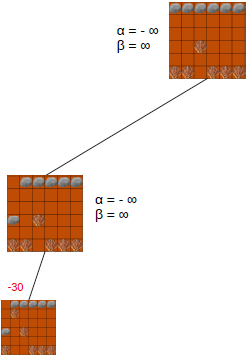
\includegraphics{img/ab1}
	\caption{Alpha-Beta: Schritt 1}
	\label{fig:ab1}
\end{figure}

\begin{figure}[h]
	\centering
	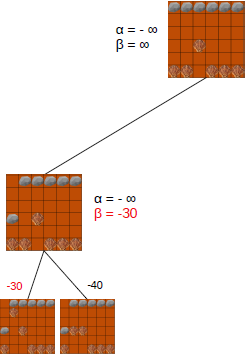
\includegraphics{img/ab2}
	\caption{Alpha-Beta: Schritt 2}
	\label{fig:ab2}
\end{figure}

\begin{figure}[h]
	\centering
	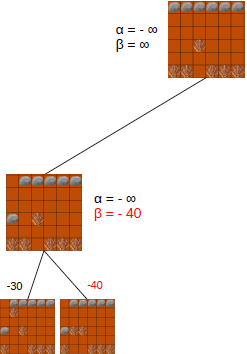
\includegraphics{img/ab3}
	\caption{Alpha-Beta: Schritt 3}
	\label{fig:ab3}
\end{figure}

\begin{figure}[h]
	\centering
	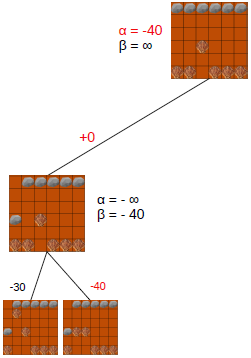
\includegraphics{img/ab4}
	\caption{Alpha-Beta: Schritt 4}
	\label{fig:ab4}
\end{figure}

\begin{figure}[h]
	\centering
	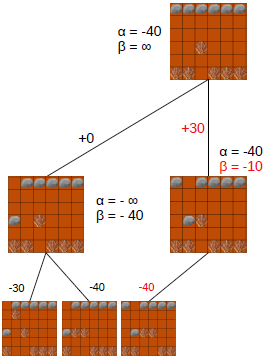
\includegraphics{img/ab5}
	\caption{Alpha-Beta: Schritt 5}
	\label{fig:ab5}
\end{figure}

\begin{figure}[h]
	\centering
	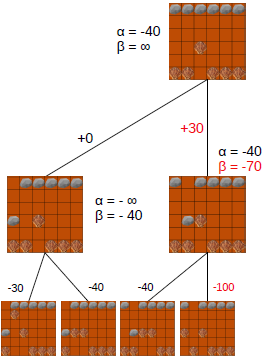
\includegraphics{img/ab6}
	\caption{Alpha-Beta: Schritt 6}
	\label{fig:ab6}
\end{figure}

\begin{figure}[h]
	\centering
	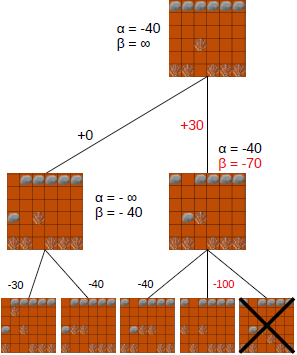
\includegraphics{img/ab7}
	\caption{Alpha-Beta: Schritt 7}
	\label{fig:ab7}
\end{figure}
\begin{figure}[h]
	\centering
	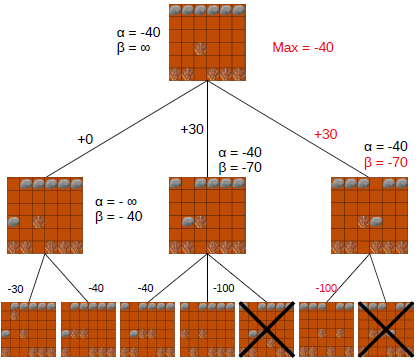
\includegraphics{img/ab8}
	\caption{Alpha-Beta: Schritt 8}
	\label{fig:ab8}
\end{figure}
%Diese Verbesserung wird dadurch erzielt, dass die Suche eines Pfades abgebrochen wird, sobald klar wird, dass das Ergebnis nicht beeinflusst wird. Als Beispiel kann die Abbildung 2.6 wieder betrachtet werden. Hier wird der linke Teilbaum zuerst durchsucht. Da jeweils vom besten Zug der Spieler ausgegangen wird, wird dieser Teilbaum durchsucht und beta wird anschließend auf -40 gesetzt (bester Zug der Muscheln). Anschließend wird der mittlere Teilbaum betrachtet. Hier wird der beste Zug der Muscheln mit -100 bewertet und somit eine neue untere Schranke von -100 festgelegt und die Durchsuchung der anderen Pfade abgebrochen, da eine bessere Wertung nicht erreichbar ist. Außerdem wird alpha mit +30 belegt. der letzte Teilbaum wird ebenfalls durchsucht bis die -100 getroffen wird und hier abgebrochen. Dadurch wird die Laufzeit verringert aber das selbe Endergebnis erzielt.



%%% Local Variables: 
%%% mode: latex
%%% TeX-master: "thesis"
%%% End: 
